%%%%%%%%%%%%%%%%%%%%%%%%%%%%%%%%%%%%%%%%%%%%%%%%%%%%%%%%%%%%%%%%%%%%%%%%%%%%%%%%%%
\begin{frame}[fragile]\frametitle{}
\begin{center}
{\Large Introduction}
\end{center}
\end{frame}

%%%%%%%%%%%%%%%%%%%%%%%%%%%%%%%%%%%%%%%%%%%%%%%%%%%%%%%%%%%%%%%%%%%%%%%%%%%%%%%%%%
\begin{frame}[fragile]\frametitle{Attribution}

Primarily based on:
\begin{itemize}
\item Gartner Hype Cycle Report 2018
\item Gartner Hype Cycle Report 2019
\item Gartner Hype Cycle Report 2020
\end{itemize}
\end{frame}

%%%%%%%%%%%%%%%%%%%%%%%%%%%%%%%%%%%%%%%%%%%%%%%%%%%%%%%%%%%%%%%%%%%%%%%%%%%%%%%%%%
\begin{frame}[fragile]\frametitle{What is a Hype Cycle?}

`` The Gartner Hype Cycle is a device that lays out the path that technologies generally take, from their initial introduction into the market until their eventual maturation into useful components of broader solutions '' - (TBD)


\begin{center}
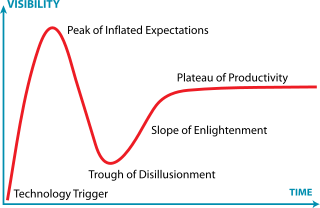
\includegraphics[width=0.4\linewidth,keepaspectratio]{gartner1}
\end{center}

{\tiny (Ref:By Jeremykemp at English Wikipedia, CC BY-SA 3.0, https://commons.wikimedia.org/w/index.php?curid=10547051)}

\end{frame}

%%%%%%%%%%%%%%%%%%%%%%%%%%%%%%%%%%%%%%%%%%%%%%%%%%%%%%%%%%%%%%%%%%%%%%%%%%%%%%%%%%
\begin{frame}[fragile]\frametitle{Phase 1: Technology Trigger}
 \begin{columns}
  \begin{column}{0.55\linewidth}
\begin{itemize}
\item When a new technology is discovered!!
\item Gets mentioned in conferences
\item Enthusiasm
\end{itemize}
  \end{column}%
  \begin{column}{0.45\linewidth}
			\begin{center}
			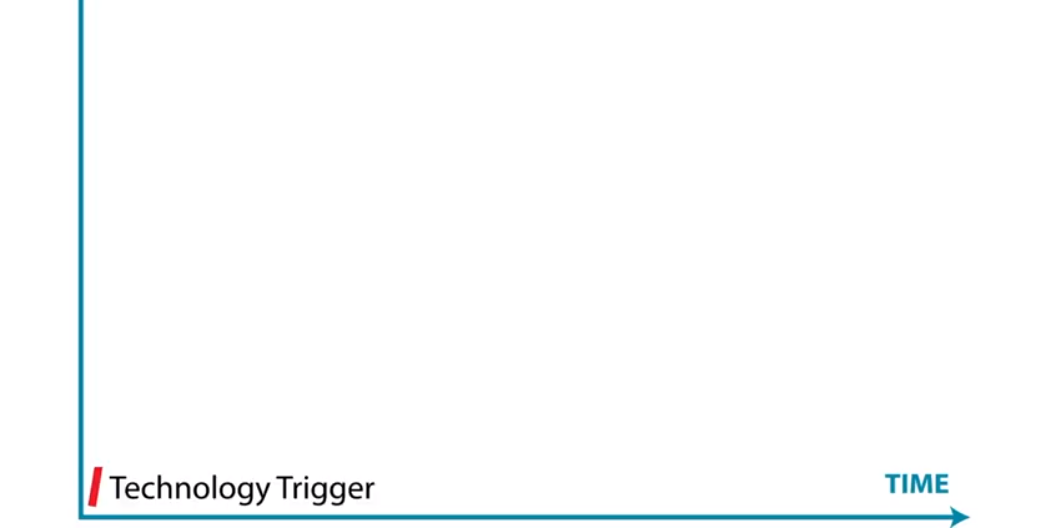
\includegraphics[width=0.9\linewidth,keepaspectratio]{gartner4}
			\end{center}
  \end{column}
 \end{columns}
 
\end{frame}

%%%%%%%%%%%%%%%%%%%%%%%%%%%%%%%%%%%%%%%%%%%%%%%%%%%%%%%%%%%%%%%%%%%%%%%%%%%%%%%%%%
\begin{frame}[fragile]\frametitle{Phase 2: Peak of Inflated Expectations}
 \begin{columns}
  \begin{column}{0.55\linewidth}
\begin{itemize}
\item Gets mentioned even in non-technical forums
\item Seen as solution for ALL problems.
\item E.g. 3D printing my dinner!!
\end{itemize}
  \end{column}%
  \begin{column}{0.45\linewidth}
			\begin{center}
			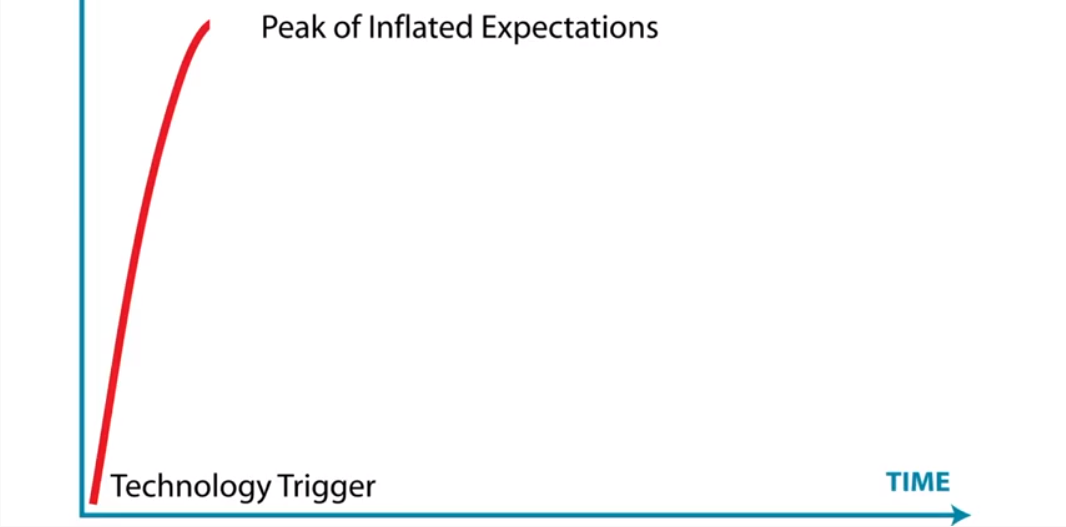
\includegraphics[width=0.9\linewidth,keepaspectratio]{gartner5}
			\end{center}
  \end{column}
 \end{columns}
 
\end{frame}

%%%%%%%%%%%%%%%%%%%%%%%%%%%%%%%%%%%%%%%%%%%%%%%%%%%%%%%%%%%%%%%%%%%%%%%%%%%%%%%%%%
\begin{frame}[fragile]\frametitle{Phase 3: Trough of Disillusionment}
 \begin{columns}
  \begin{column}{0.55\linewidth}
\begin{itemize}
\item Does not live up to ALL expectations
\item Disillusionment
\item Some die here!!
\end{itemize}
  \end{column}%
  \begin{column}{0.45\linewidth}
			\begin{center}
			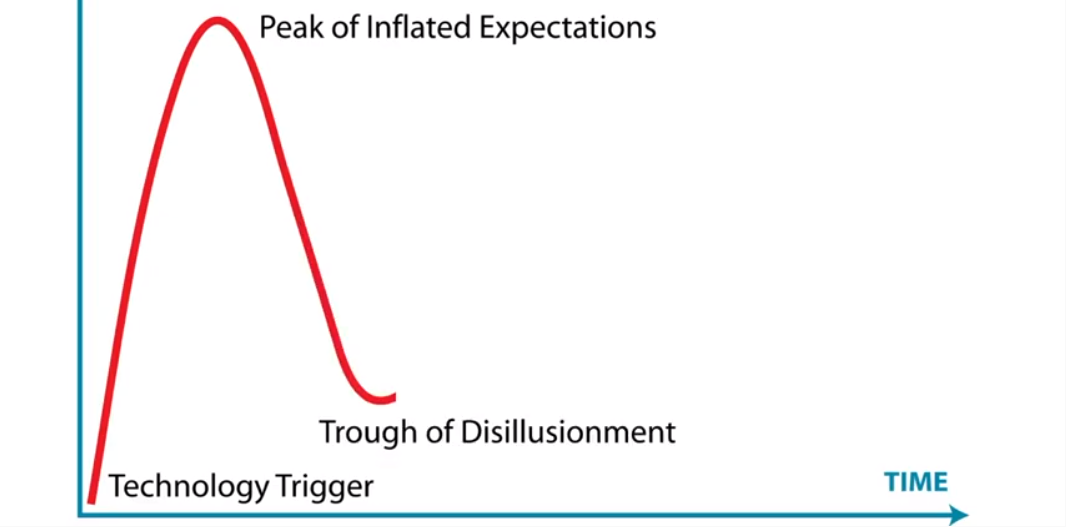
\includegraphics[width=0.9\linewidth,keepaspectratio]{gartner6}
			\end{center}
  \end{column}
 \end{columns}
 
\end{frame}

%%%%%%%%%%%%%%%%%%%%%%%%%%%%%%%%%%%%%%%%%%%%%%%%%%%%%%%%%%%%%%%%%%%%%%%%%%%%%%%%%%
\begin{frame}[fragile]\frametitle{Phase 4: Scope of Enlightenment}
 \begin{columns}
  \begin{column}{0.55\linewidth}
\begin{itemize}
\item Those who survive the trough
\item May not solve ALL the problems but some specific ones.
\item Focused development
\end{itemize}
  \end{column}%
  \begin{column}{0.45\linewidth}
			\begin{center}
			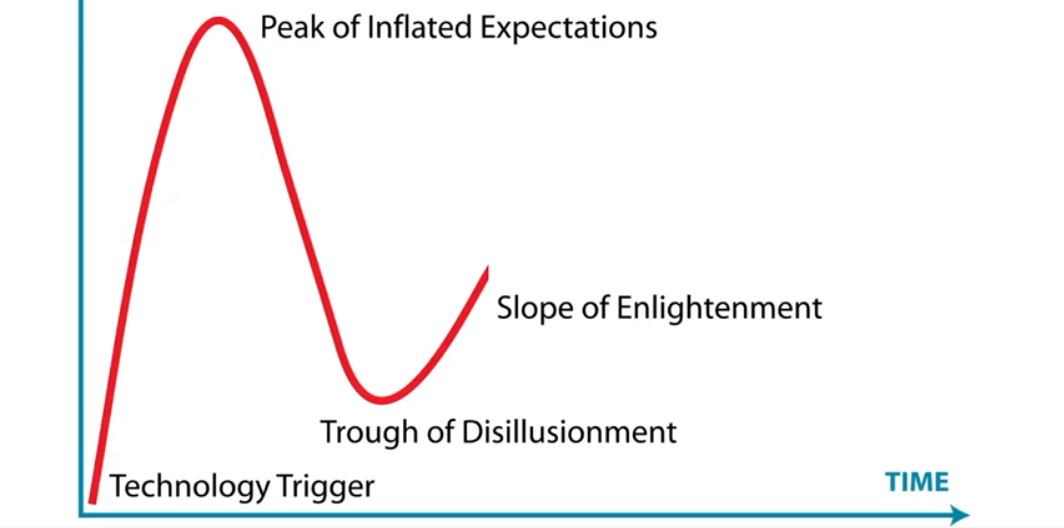
\includegraphics[width=0.9\linewidth,keepaspectratio]{gartner7}
			\end{center}
  \end{column}
 \end{columns}
 
\end{frame}


%%%%%%%%%%%%%%%%%%%%%%%%%%%%%%%%%%%%%%%%%%%%%%%%%%%%%%%%%%%%%%%%%%%%%%%%%%%%%%%%%%
\begin{frame}[fragile]\frametitle{Phase 5: Plateau of Productivity}
 \begin{columns}
  \begin{column}{0.55\linewidth}
\begin{itemize}
\item Good, mature products
\item Survives longer
\end{itemize}
  \end{column}%
  \begin{column}{0.45\linewidth}
			\begin{center}
			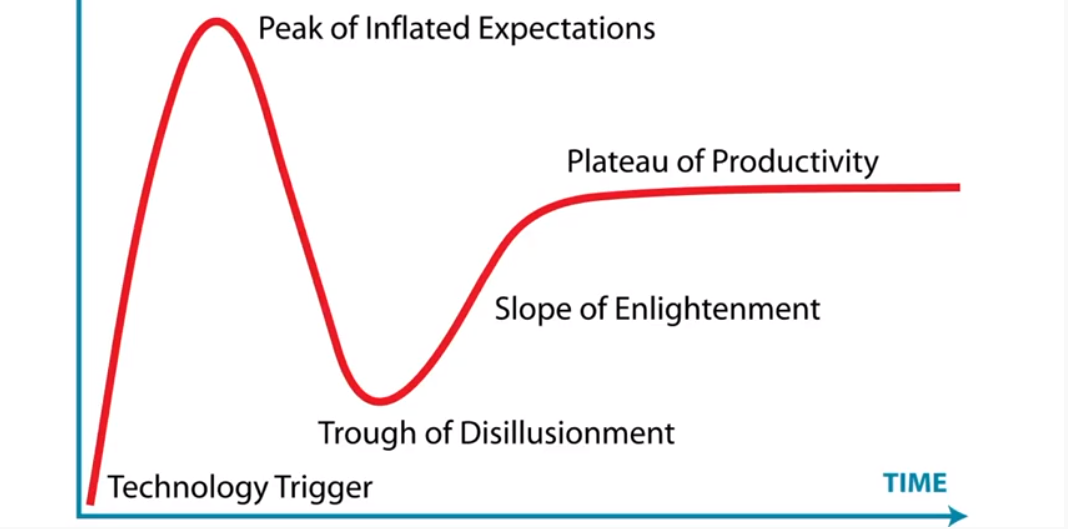
\includegraphics[width=0.9\linewidth,keepaspectratio]{gartner8}
			\end{center}
  \end{column}
 \end{columns}
 
\end{frame}


%%%%%%%%%%%%%%%%%%%%%%%%%%%%%%%%%%%%%%%%%%%%%%%%%%%%%%%%%%%%%%%%%%%%%%%%%%%%%%%%%%
\begin{frame}[fragile]\frametitle{Summary : Phases}

\begin{center}
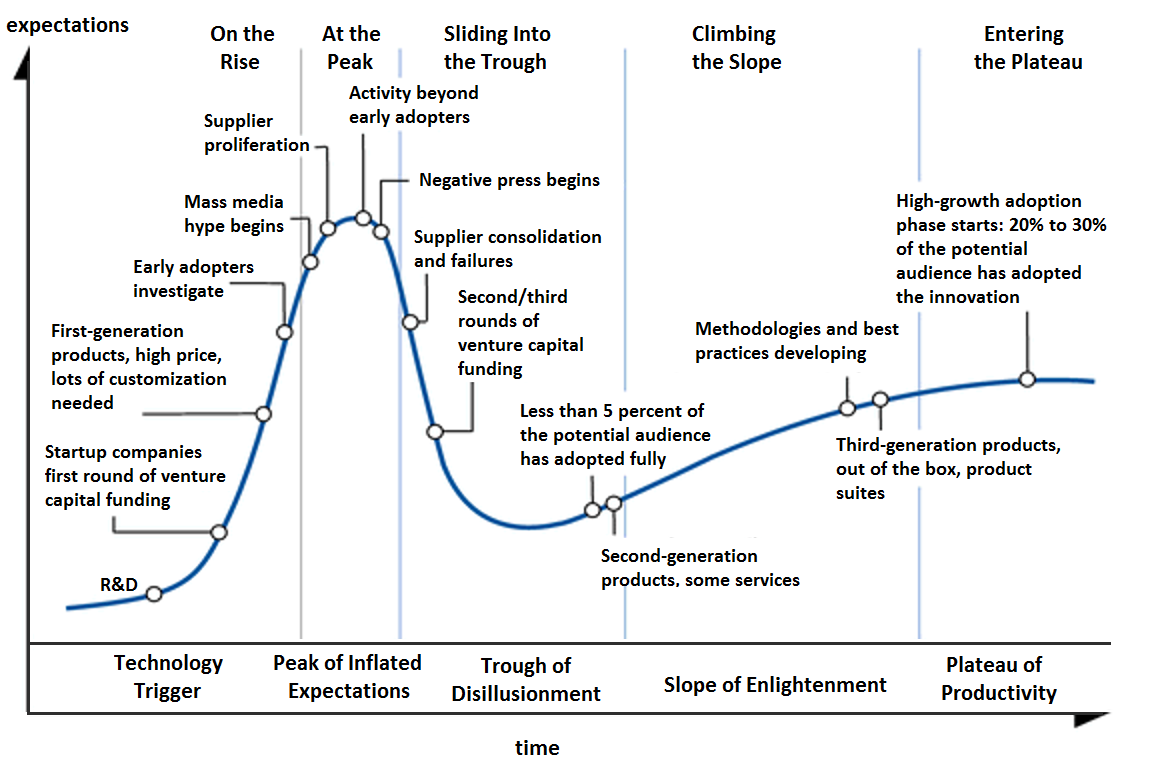
\includegraphics[width=0.8\linewidth,keepaspectratio]{gartner2}
\end{center}

{\tiny (Ref: By NeedCokeNow - Own work, CC BY-SA 3.0, https://commons.wikimedia.org/w/index.php?curid=27546041)}
\end{frame}

%%%%%%%%%%%%%%%%%%%%%%%%%%%%%%%%%%%%%%%%%%%%%%%%%%%%%%%%%%%%%%%%%%%%%%%%%%%%%%%%%%
\begin{frame}[fragile]\frametitle{What it is for?}

``Clients use Hype Cycles to get educated about the promise of an emerging technology within the context of their industry and individual appetite for risk.''

- Gartner 


\end{frame}

%%%%%%%%%%%%%%%%%%%%%%%%%%%%%%%%%%%%%%%%%%%%%%%%%%%%%%%%%%%%%%%%%%%%%%%%%%%%%%%%%%
\begin{frame}[fragile]\frametitle{History of Gartner Hype Cycles?}


\end{frame}

%%%%%%%%%%%%%%%%%%%%%%%%%%%%%%%%%%%%%%%%%%%%%%%%%%%%%%%%%%%%%%%%%%%%%%%%%%%%%%%%%%
\begin{frame}[fragile]\frametitle{Trends in 2018}



\end{frame}

%%%%%%%%%%%%%%%%%%%%%%%%%%%%%%%%%%%%%%%%%%%%%%%%%%%%%%%%%%%%%%%%%%%%%%%%%%%%%%%%%%
\begin{frame}[fragile]\frametitle{Trends in 2019}

\begin{center}
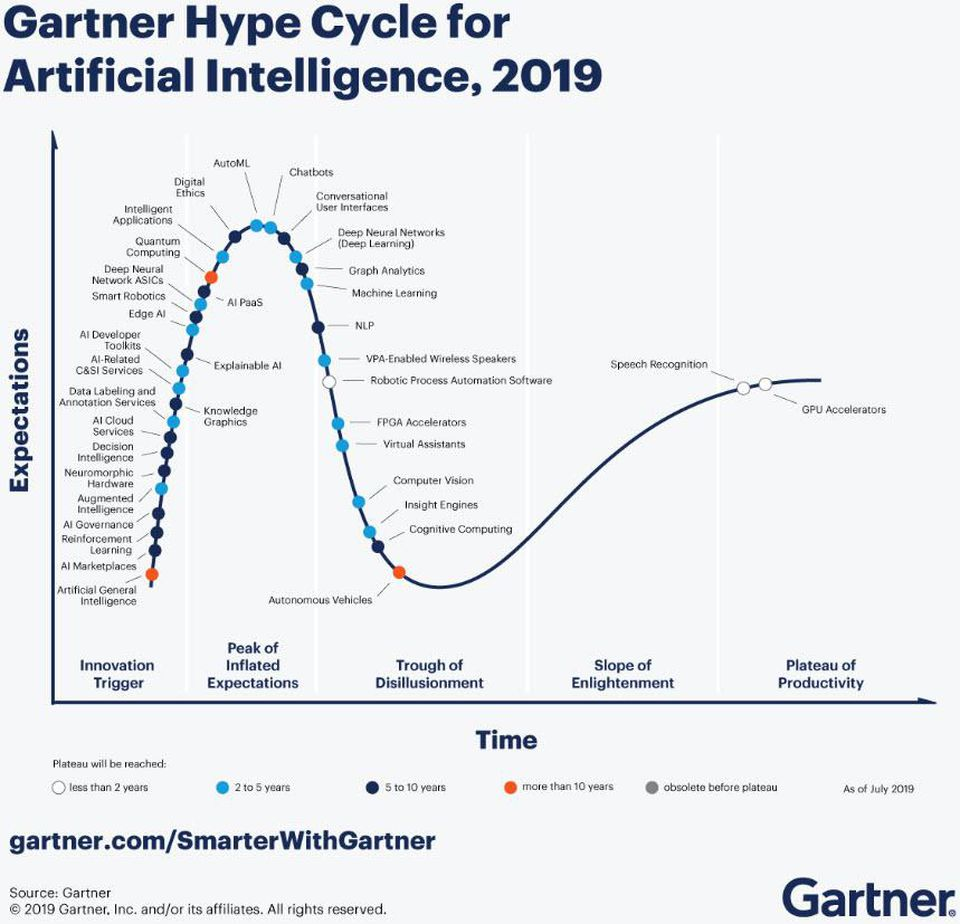
\includegraphics[width=0.7\linewidth,keepaspectratio]{gartner3}
\end{center}

\end{frame}

%%%%%%%%%%%%%%%%%%%%%%%%%%%%%%%%%%%%%%%%%%%%%%%%%%%%%%%%%%%%%%%%%%%%%%%%%%%%%%%%%%
\begin{frame}[fragile]\frametitle{Trends in 2020}



\end{frame}

%%%%%%%%%%%%%%%%%%%%%%%%%%%%%%%%%%%%%%%%%%%%%%%%%%%%%%%%%%%%%%%%%%%%%%%%%%%%%%%%%%
\begin{frame}[fragile]\frametitle{Transitions}



\end{frame}



%%%%%%%%%%%%%%%%%%%%%%%%%%%%%%%%%%%%%%%%%%%%%%%%%%%%%%%%%%%%%%%%%%%%%%%%%%%%%%%%%%
\begin{frame}[fragile]\frametitle{Criticism By Patrick Crouch}


\begin{itemize}
\item Personally, couldn’t find a single example of tech-oriented company using the Hype Cycle to determine spending or strategy.
\item So who’s using it? Answer: Marketers.
\item Most technological advances come from the combination or misuse of a variety of technologies, not from one technology being researched
\item The Gartner Hype Cycle is more of a scapegoat for failing/unrealized technical promise than a useful tool

\end{itemize}

{\tiny (Ref: The Gartner Hype Cycle - Does the Gartner Hype Cycle Invalidate Itself? - By: Patrick Crouch)}

\end{frame}


%%%%%%%%%%%%%%%%%%%%%%%%%%%%%%%%%%%%%%%%%%%%%%%%%%%%%%%%%%%%%%%%%%%%%%%%%%%%%%%%%%
\begin{frame}[fragile]\frametitle{}
\begin{center}
{\Large Conclusion}
\end{center}
\end{frame}



%%%%%%%%%%%%%%%%%%%%%%%%%%%%%%%%%%%%%%%%%%%%%%%%%%%%%%%%%%%%%%%%%%%%%%%%%%%%%%%%%%
\begin{frame}[fragile]\frametitle{Additional References}


\begin{itemize}
\item What's New In Gartner's Hype Cycle For AI, 2019 - Louis Columbus
\item Gartner Hype Cycle - J Scott Christianson
\end{itemize}

\end{frame}

% %%%%%%%%%%%%%%%%%%%%%%%%%%%%%%%%%%%%%%%%%%%%%%%%%%%%%%%%%%%%%%%%%%%%%%%%%%%%%%%%%%
% \begin{frame}[fragile]{Evolution of CAD Technology}
% \begin{center}
% \includegraphics[width=0.9\linewidth,keepaspectratio]{geomod1}
% \end{center}
% \end{frame}

% %%%%%%%%%%%%%%%%%%%%%%%%%%%%%%%%%%%%%%%%%%%%%%%%%%%%%%%%%%%%%%%%%%%%%%%%%%%%%%%%%%
% \begin{frame}[fragile]{Manual drafting}
 % \begin{columns}
  % \begin{column}{0.55\linewidth}
% \begin{itemize}
% \item 2D representations used to represent 3D objects
% \begin{itemize}
% \item multi-view drawings
% \item pictorials
% \end{itemize}
% \item Standards and conventions developed so that 3D object could be built from drawings
% \item Drawings created manually or using 2D CAD
% \item Difficult to visualize, error-prone, time-consuming
% \end{itemize}
  % \end{column}%
  % \begin{column}{0.45\linewidth}
			% \begin{center}
			% \includegraphics[width=0.9\linewidth,keepaspectratio]{geomod2}
			% \end{center}
  % \end{column}
 % \end{columns}
% \end{frame}

